\documentclass[conference]{InputFiles/IEEEtran}

% % % % % % % % % % package starts...% % % % % % % % % % % % % % % % % % % % %
	\usepackage{graphicx}
	\usepackage{balance}
	\usepackage{amssymb, amsmath, amsthm}
	\usepackage{multirow, rotating, wasysym, url}
	\usepackage[tight]{subfigure}
	%\usepackage[retainorgcmds]{InputFiles/IEEEtrantools}
	\usepackage[ruled,linesnumbered,vlined]{algorithm2e}
	\usepackage{hyperref} %reference hyper links.
	\usepackage{color}
  %\usepackage{algorithm}
  % \usepackage{algorithmic}
  \usepackage{algpseudocode}
%  \usepackage{mathcal}
 %   \usepackage{amsmath}
% % % % % % % % % % package ends...% % % % % % % % % % % % % % % % % % % % % %


\graphicspath{{./DrawingFigures/},{./EvaluateFigures/}}

% % % % % % % % % % New command starts...% % % % % % % % % % % % % % % % % % 
	\newcommand{\presec}{\vspace{-0in}}
	\newcommand{\postsec}{\vspace{-0in}}
	\newcommand{\presub}{\vspace{-0in}}
	\newcommand{\postsub}{\vspace{-0in}}
	\newcommand{\precaption}{\vspace{-0in}}
	\newcommand{\postcaption}{\vspace{-0in}}
	\newcommand{\preequation}{\vspace{-0in}}
	\newcommand{\postequation}{\vspace{-0in}}
	\newcommand{\prefig}{\vspace{-0in}}
	\newcommand{\prefigcaption}{\vspace{-0in}}
	\newcommand{\postfig}{\vspace{-0in}}
	\newcommand{\subfigs}{\hspace{-0in}}
	\newcommand{\subfigsvert}{\vspace{-0in}}
	\newcommand{\pretheorem}{\vspace{-0in}}
	\newcommand{\posttheorem}{\vspace{-0in}}
		\mathchardef\Gamma="0100 \mathchardef\Delta="0101
\mathchardef\Theta="0102 \mathchardef\Lambda="0103
\mathchardef\Xi="0104 \mathchardef\Pi="0105
\mathchardef\Sigma="0106 \mathchardef\Upsilon="0107
\mathchardef\Phi="0108 \mathchardef\Psi="0109
\mathchardef\Omega="010A

\newcommand{\ovspace}[1]{\vspace{#1}}

\newcommand{\outline}[1]{}%{\textbf{#1}}

\newcommand{\dl}{\mbox{$\, [ \hspace*{-1.5pt} [\,$}}
\newcommand{\dr}{\mbox{$\, ] \hspace*{-1.5pt} ]\:$}}
\newcommand{\da}{\mbox{$\, A \hspace*{-6.75pt} A \,$}}
%\newcommand{\drightarrow}{\mbox{$\rightarrow \hspace*{-8pt} \rightarrow$}}

\newcommand{\BA}{\mbox{${\bm{a}}$}}
%\newcommand{\BB}{\mbox{${\bm{c}}$}}
\newcommand{\BC}{\mbox{${\bm{c}}$}}
\newcommand{\BD}{\mbox{${\bm{d}}$}}
\newcommand{\BE}{\mbox{${\bm{e}}$}}
\newcommand{\BO}{\mbox{${\bm{o}}$}}
\newcommand{\BP}{\mbox{${\bm{p}}$}}
\newcommand{\BQ}{\mbox{${\bm{q}}$}}
\newcommand{\BR}{\mbox{${\bm{r}}$}}
\newcommand{\BV}{\mbox{${\bm{v}}$}}
\newcommand{\BL}{\mbox{${\bm{l}}$}}
\newcommand{\BI}{\mbox{${\bm{i}}$}}
\newcommand{\BH}{\mbox{${\bm{h}}$}}
\newcommand{\BS}{\mbox{${\bm{s}}$}}
\newcommand{\BB}{\mbox{${\bm{k}}$}}

\newcommand{\wrapbox}[1]{\framebox{\begin{tabular}{c}#1\end{tabular}}}
\newcommand{\CodeIn}[1]{{\small\texttt{#1}}}
\newcommand{\Section}[1]{Section~\ref{sec:#1}}
\newcommand{\SFigure}[2]{Figure~\ref{fig:#1}(#2)}

\usepackage{cite}
\usepackage{xspace}
\usepackage{url}
\usepackage{graphicx}
\usepackage{latexsym}
\usepackage{amssymb}
\usepackage{amsfonts}
%\usepackage{times}
\usepackage{psfrag}
%\usepackage{subfigure}
\usepackage{wrapfig}
\usepackage{comment}
%packages for algorithms
%\usepackage{algorithm}
%\usepackage{algorithmic}
\usepackage{alltt}
\usepackage{color}

\newtheorem{defn}{Definition}[section]
\newtheorem{exmp}{Example}[section]
\newtheorem{thrm}{Theorem}[section]
\newtheorem{prop}{Proposition}[section]
\newtheorem{lemm}{Lemma}[section]
\newtheorem{obsv}{Observation}[section]
\newtheorem{corr}{Corollary}[section]

%\addtolength{\textheight}{.23in} \addtolength{\textwidth}{.15in}
%\addtolength{\topmargin}{-.23in}
%\addtolength{\oddsidemargin}{.1in}
%\addtolength{\evensidemargin}{.1in}

\newtheorem{thm}{Theorem}
\newtheorem{dfn}{Definition}
\newtheorem{lem}{Lemma}
\newtheorem{cor}{Corollary}
\newcommand{\ie}{\emph{i.e.}\xspace}
\newcommand{\eg}{\emph{e.g.}\xspace}
\newcommand{\etc}{\emph{etc.}\xspace}
\newcommand{\etal}{\frenchspacing{}\emph{et al{.}}\xspace}
%\newcommand{\etal}[1]{{\sl et al.{#1}}}

%\newcommand{\thm}[1]{Theorem~\ref{thm:#1}}
%\newcommand{\lem}[1]{Lemma~\ref{lemma:#1}}
%\newcommand{cor}[1]{Corollary~\ref{cor:#1}}
\newcommand{\fac}[1]{Fact~\ref{fact:#1}}
\newcommand{\Table}[1]{Table~\ref{tab:#1}}
\newcommand{\Figure}[1]{Figure~\ref{fig:#1}}

%\theoremstyle{plain}
\newtheorem{property}{Property}[section]
\newtheorem{lemma}{Lemma}[section]
\newtheorem{corollary}{Corollary}[section]
\newtheorem{theorem}{Theorem}[section]

%\theoremstyle{definition}
\newtheorem{notation}{Notation}
\newtheorem{Definition}{Definition}[section]

%\theoremstyle{remark}
\newtheorem{fact}{Fact}[section]
\newtheorem{observation}{Observation}[section]
\newtheorem{insight}{Insight}[section]

%%\algorithmstyle{definition}
%\algsetup{indent=1em}
%\renewcommand{\algorithmicrequire}{\textbf{Input:  }}
%\renewcommand{\algorithmicensure}{\textbf{Output:}}
\newcommand{\factorial}{\ensuremath{\mbox{\sc Factorial}}}

%\newcommand{\Comment}[1]{}

\renewcommand\floatpagefraction{0.999}
\renewcommand\topfraction{0.999}
\renewcommand\bottomfraction{0.999}
\renewcommand\textfraction{0.001}
\setcounter{totalnumber}{5}

		\newcommand{\Proc}{Proc. }
		\newcommand{\Conf}{Conf. }
		\newcommand{\Inte}{Int. }
		\newcommand{\Symp}{Symp. }
	\newcommand{\tabincell}[2]{\begin{tabular}{@{}#1@{}}#2\end{tabular}}
	
	\newcommand{\figwidthdraw}{0.45\textwidth}
	\newcommand{\figwidtheva}{0.4\textwidth}
	\newcommand{\aname}{CDV}
	\newcommand{\fname}{HC}
	\newcommand{\ccm}{C$_\text{CM}$ sketch}

	
	\definecolor{greener}{RGB}{0,166,0}
	\definecolor{reder}{RGB}{255,0,0}
	\definecolor{bluer}{RGB}{0,0,255}
	
	\clubpenalty=10000
	\widowpenalty = 10000
% % % % % % % % % % New command ends...% % % % % % % % % % % % % % % % % % % %

% % % % % % % % % % Backup starts... % % % % % % % % % % % % % % % % % % % % %
	%\clubpenalty=10000
	%\widowpenalty = 10000
	%\usepackage{caption2} %fo setlength
	%\setlength{\parskip}{0.1\baselineskip}
	%\setlength{\abovecaptionskip}{-1pt}
	%\vfill\eject % force going to next page
% % % % % % % % % % Backup ends... % % % % % % % % % % % % % % % % % % % % % %
	
\title{\fname: Better Parameter Settings for Sketches without Extra Costs}

\title{\fname: A Probablistic Data Structure for Single Set Queries, Multiple Set Queries, and Multiset Queries}

\author{Paper \#101, 6 pages}

\begin{document}
\maketitle
\sloppy
%\Comment
	
	\begin{abstract}
	Sketch is a probabilistic data structure used to record frequencies of items in a multiset.
	It can work with small memory usage and achieve high speed and accuracy.
	Therefore, sketches have been widely used in many applications, such as data stream processing, distributed datasets, natural language processing, and network traffic analysis.
	However, conventional sketches are not accurate enough for non-uniform datasets, which are common in practice.
	In this paper, we propose a novel technique, named \fname~(\aname), which can improve the accuracy of sketches for non-uniform datasets without extra costs.
	The key idea of our technique is to use different parameters, including width and counter size, for different arrays in a sketch.
	We applied our novel technique to several well-known sketches, including CM sketches and CU sketches.
	We also made mathematical analysis to prove that our technique is able to improve the accuracy of sketches.
	Extensive experimental results show that our \aname~has improved the accuracy of existing sketches by up to ...
	The source codes of our new technique are available on our homepage.
\end{abstract}
	\presec
\section{Introduction} \postsec

\presub
\subsection{Background and Motivation} \postsub

There are three fundamental problems in computer science: single set queries, multiple set queries, and multiset queries. 
1) \texttt{Single set queries:} Given a set $\mathcal{S}$ and an element $e$, does $e$ belongs to $\mathcal{S}$? This is the problem of . 2) \texttt{Multiple set queries:} Given z sets and an element $e$, which set(s) contains $e$? 
3) \texttt{Multiset queries:} Given a multiset $\mathcal{S'}$ and an element $e$, how many times does $e$ appears in $\mathcal{S'}$, and what are the top-$k$ frequent items? 
A multiset refers to a set in which an item can appear more than once.
Due to the significance of these three kinds of queries, multiple solutions have been proposed to address each kinds of queries.
However, all existing solutions are designed for only one specific query.
The design goal of this paper is to propose one data structure which can be used to address all these three kinds of queries. 





In today's computer science, estimating the frequency of items in a multiset is a very important problem.
A multiset is a set in which items can appear more than once.
This problem has been studied in various of fields, such as data stream processing \cite{charikar2002finding,aggarwal2010on,manerikar2009frequent,thomas2009on}, network traffic analysis \cite{liu2016one,chen2010tracking}, natural language processing (NLP) \cite{goyal2012sketch,goyal2009streaming}, data graph \cite{zhao2011gsketch:}, distributed databases \cite{cormode2005sketching}, social network \cite{aggarwal2012event}, \etc
As the speed of data streams becoming faster and faster, it becomes more difficult to achieve accurate estimation for item frequencies, and thus many approximate approaches using probabilistic data structures are being widely used and studied.
Among all these approximate approaches, sketches \cite{sketchsurvey} are considered the most successful one due to their high accuracy and fast speed.

A sketch is a probabilistic data structure that can be used to store the frequencies of items in a multiset. 
Compared to other methods for frequency query, sketches are more memory efficient and can achieve faster speed and higher accuracy.
Therefore, sketches are widely used for the problem of estimating item frequencies.
%Therefore, sketches are widely used in various kinds of applications, such as data stream processing, distributed datasets, natural language processing, and network traffic analysis.
Typical sketches include CM sketches \cite{cormode2005an} and CU sketches \cite{estan2001new}. A CM sketch consists of $d$ arrays, $A_1, A_2 \dots A_d$, and each array consists of $w$ counters. Furthermore, each array is associated a hash function $h_i(.) (1\leqslant i\leqslant d)$.
When inserting an item $e$, the CM sketch first computes these $d$ hash functions, $h_1(e), h_2(e) \dots h_d(e)$, and maps the item to $d$ counters, $A_1[h_1(e)], A_2[h_2(e)] \dots A_d[h_d(e)]$. Then it increments these $d$ mapped counters by 1.
When querying an item $e$, the CM sketch just reports the minimum value from these $d$ mapped counters.
The CU sketch has the same structure and query process as the CM sketch, but it only increments the mapped counters with minimum values instead of incrementing all of them when performing insertion processes.
According to the analysis of real datasets, we found that most real datasets are non-uniform, which means that in most datasets, most items have a small frequency, while only a few items have a high frequency.
For convenience, we call items with a small frequency \texttt{cold items}, and those with a high frequency \texttt{hot items}.
However, all conventional sketches are unable to deal with this issue, because they are difficult to find a proper counter size to fit these non-uniform datasets.
Therefore, there are many counters containing a small number (typically less than 10), and it is definitely a waste of memory.
With a fixed memory size, the accuracy of sketches could be poor due to the big waste of memory.

To address this issue, there are many improved approaches, such as Augmented sketch (ASketch) \cite{roy2016augmented}, Counter Braids (CB) \cite{lu2008counter}, \etc
The ASketch adds a filter to a CM sketch, which contains frequencies for a certain number of \texttt{hot items}.
Therefore, the ASketch achieves higher accuracy than conventional sketches in terms of \texttt{hot items}.
However, the average accuracy of all items is not improved.
The Counter Braids can dynamically allocate more counter size for \texttt{hot items}, and can achieve 100\% accuracy in most cases.
However, the Counter Braids does not support instant query, which means we can only query the frequencies of items after inserting all items.
Note that prior approaches still have some shortcomings as mentioned above.
To address this issue, we propose a novel technique, which can enable sketches perform better on these non-uniform datasets without extra costs like more memory accesses or more computations.
%Note that prior approaches still have some shortcomings, and only focus on \texttt{hot items}.
%However, we claim that in many applications, \texttt{cold items} are as important as \texttt{hot items}, and thus we cannot simply overlook their existence.
%For example, ...
%However, most prior approaches have poor performance on these \texttt{cold items}.
%To address this issue, we propose a novel technique, which can enable sketches perform better on these non-uniform datasets without extra costs like more memory accesses and more computation.

\presub
\subsection{Proposed Approach} \postsub

In this paper, we propose a novel technique for sketches, named \fname~(\aname), which enables sketches to perform better accuracy on non-uniform datasets without extra costs.
\textit{One of the key principles of our \aname~technique is to use different parameters, including width and counter size, for different arrays in a sketch.}
To be specific, we use geometric progression to generate counter sizes for arrays in the sketch.
For example, we use a counter size of 2 bits for the first array, 4 bits for the second array, 8 bits for the third array, \etc
%Usually, a sketch has 4 arrays and a counter size of 16 bits is enough to contain the maximum frequency among all items.
A sketch usually has 4 arrays, and a counter size of 16 bits is enough to contain the maximum frequency among all items.
Furthermore, we also use different width for each array, and typically we set a larger width for the array with smaller counter size.
Note that in most real datasets, most items have a small frequency (about half of items have a frequency no larger than 2).
The larger width for the array with smaller counter size has two following advantages: 1) it saves memory usage because the counter size is small. 2) it reduces the probability of hash collisions, and thus enhances the accuracy significantly.
%Therefore, the accuracy of all items increases.

\textit{The second principle of our \aname~technique is to treat counter overflows as flags that indicates the counter is mapped by items with larger frequencies than the capacity of the counter.}
As stated above, we may use a counter size of only 2 bits for the first array, and thus counter overflows will happen frequently in this array.
If we simply treat these overflowed counters as usual, then we will get illogical results.
For example, if we apply our \aname~technique to a CM sketch, when querying an arbitrary item, we can only get an estimated result smaller than 4, and then errors of \texttt{hot items} will be very huge.
Therefore, we should treat counter overflows differently: we simply ignore these overflowed values, and do not take these values into account when performing query processes.

There are two important advantages of our \aname~technique:
1) our \aname~technique can significantly increase the accuracy for non-uniform datasets.
2) our \aname~technique will introduce few extra costs, such as more computational cost, more memory accesses, \etc

\presub
\subsection{Key Contributions} \postsub

\begin{enumerate}
	\item First, we propose a novel technique for sketches, named \fname~(\aname), which can significantly increase the accuracy of sketches on non-uniform datasets with few extra costs.
	\item Second, we carry out comprehensive mathematical analysis and extensize experiments, and the results prove that our \aname~has a great advantage over conventional sketches and the state-of-the-art in terms of accuracy.
	\item Third, we place all related source codes of our \aname~technique at our homepage.
\end{enumerate}
	\presec
\section{Related Work} \postsec

As data stream processing becomes more and more important these days, it becomes more difficult for conventional approaches to work at a high speed. Therefore, many approaches have been proposed in recent years, including sketches and counter variants.

The CM and CU sketch have been introduced in the previous section. To overcome the limitations of these conventional sketches, several improvements are proposed. For example, the Augmented Sketch (ASketch) \cite{roy2016augmented} is proposed by Roy \etal
An ASketch consists of a conventional CM sketch and a filter that contains frequencies for \texttt{hot items}.
When inserting an item $e$, it first checks whether $e$ is in the filter.
If so, it directly increments the corresponding counter in the filter by 1. Otherwise, it inserts it into the CM sketch.
After each insertion, it will reorganize the filter to guarantee the items with highest frequencies are in the filter.
%The Count-min-log sketch (CML sketch) \cite{cmlsketch} is proposed by Pitel \etal
%It solves the problem of counter overflows.
%Different from the CM sketch, the CML sketch uses logarithm-based approximate counters rather than linear counters. It increments its counters with logarithmic probabilities instead of incrementing in all cases.
%Therefore, counters in the CML sketch are able to contain a much larger frequency.
%However, all these approaches have significant shortcomings.
However, the ASketch only achieves higher accuracy for a certain number of \texttt{hot items}, but does not enhance the overall accuracy of all items.
%The CML sketch introduces bigger errors when storing large frequencies.

There are also several counter-based approaches aiming to solve the problem faced by conventional sketches.
The most typical one is the Counter Braids \cite{lu2008counter}.
The Counter Braids uses a layered structure.
When inserting \texttt{cold items}, it only increments the counters in the first layer.
While when inserting \texttt{hot items}, counters in the first layer may overflow and those in deeper layers will be incremented.
The Counter Braids can achieve 100\% accuracy in most cases, and is also memory efficient.
However, it does not support instant query, which means that we can only query the item frequencies after inserting all items.

%Furthermore, most of these approaches stated above mainly focus on \texttt{hot items}.
%However, in many applications \texttt{cold items} are as important as \texttt{hot items}.
As mentioned above, all these approaches have obvious shortcomings, including low overall accuracy, not supporting certain functions, \etc
Therefore, these approaches may have poor performance in their applications.
The design goal of our proposed technique is to enhance the overall accuracy for sketches with few extra costs.

	\presec
\section{The \fname~Technique} \postsec

In this section, we present the details of our \fname~technique which can be applied to all exisiting sketches.
We mainly present two key techniques of our \fname: \textit{unbalanced parameter setting and overflow skip}.
By applying the unbalanced parameter setting technique, we can increase the width of arrays with a small counter size, which can significantly reduce the probability of hash collisions.
Therefore, the overall accuracy can be improved. %and thus significantly enhance the accuracy of \texttt{cold items}.
%By applying the overflow skip technique, we can guarantee the accuracy of \texttt{hot items} keeping at a high level.
By applying the overflow skip technique, we can prevent the illogical results for some items.
Table \ref{table:symbols} summarizes the symbols and abbreviations used in this paper.

\begin{table}[htbp]
	\centering
	\caption{Symbols \& abbreviations used in the paper}
	\begin{tabular}{|c|l|}
		\hline
		\textbf{Symbol}&\textbf{Description}\\
		\hline
		$d$& \# of arrays of a sketch\\
		\hline
		$w_i$& \# of counters in the $i^{th}$ array\\
		\hline
		$\overline{w}_i$& \# of bits in the $i^{th}$ array\\
		\hline
		$b_i$& the counter size in the $i^{th}$ array\\
		\hline
		$e$& an arbitrary element\\
		\hline
		A$_i$& the $i^{th}$ array in a sketch\\
		\hline
		A$_i$[$j$]& the counter in the $j^{th}$ position of the $i^{th}$ array\\
		\hline
		$h_i(.)$& the $i^{th}$ hash function\\
		\hline
		CR& the correct rate of a sketch\\
		\hline
		RE& the relative error of an item\\
		\hline
		AE& the absolute error of an item\\
		\hline
		ARE& the average relative error of a sketch\\
		\hline
		AAE& the average absolute error of a sketch\\
		\hline
		Mips& mega-instructions per second\\
		\hline
	\end{tabular} 
	\label{table:symbols}
\end{table}

\presub
\subsection{Technique I: Unbalanced Parameter Setting} \postsub

\presub
\subsubsection{Rationale} \postsub

As stated above, in most real datasets, most items have a small frequency (typically less than 10), and only a few items have a large frequency. 
%Prior approaches mainly focus on \texttt{hot items}, and achieve higher accuracy of these items. Here we claim that \texttt{cold items} are also important, since the percentage of \texttt{cold items} is much larger than that of \texttt{hot items}.
Conventional sketches use the same parameters for each array, but this parameter setting could wastes a lot of memory since most items have a small frequency, while the counter size should be large enough to contain the largest frequency among all items in the data stream.
Therefore, with fixed memory size, the width of each array can be quite small, and thus more hash collisions will happen, leading to a low overall accuracy.
%Therefore, we should use different parameters for different arrays.
So using different parameters for different arrays is a wise solution.
On the one hand, we can set a smaller counter size for some arrays, and thus we can also set a larger width for these arrays.
It can significantly reduce the probability of hash collisions for these arrays, and therefore improve the arruacy.
On the other hand, we should also set a big counter size for some other arrays, since we should have counters whose size is big enough to contain large frequencies.
Furthermore, the width of these arrays do not need to be large, since the percentage of items with large frequencies is small.
Therefore, it can also guarantee the accuracy of \texttt{hot items}.
Sketches using our unbalanced parameter setting technique may take on different structures. Here we mainly introduce two versions of our technique.

\presub
\subsubsection{Version 1} \postsub

Based on conventional sketches like CM sketches, we first set different counter sizes for different arrays in the first version.

\noindent\textbf{Technical content: }As the name of our technique indicates, the first version of our technique uses the idea of cell division.
There are two main points to present this version: 1) it uses the same amount of memory (same number of bits) for each array, like conventional sketches; 2) it uses different counter size for each array. For example, there are 4 arrays in a sketch, and it uses a counter size of 2 bits, 4 bits, 8 bits and 16 bits for the 4 arrays. Therefore, if the width of the fourth array is $w$, then the first three arrays has a width of $8w$, $4w$, and $2w$, respectively.
Assume that each counter is a cell, and each division will transform one single bigger cell into two smaller cells.
Then counters in the first array have experienced cell division for three rounds, and those in the second and the third array have experienced for two rounds and one round, respectively. Furthermore, the total number of bits keeps constant after each round of division, which resembles the substance conservation phenomenon in cell divisions.
The structure of this example is shown in Figure \ref{draw:version1}.

\noindent\textbf{Analysis: }As stated above, arrays with a small counter size reduces the probability of hash collisions, and thus increase the accuracy significantly. Arrays with a large counter size is able to contain the large item frequencies, and can prevent large errors for items with large frequencies. Therefore, the overall accuracy of the data stream can be enhanced greatly. However, this parameter setting for sketches may not be the best in many cases.
Assume that there are only about 10\% \texttt{cold items} whose frequency is less than 3, then most counters in the array whose counter size is 2 bits will overflow. It will waste a large amount of memory usage, and the performance is not good enough.
In the next version, we will solve this issue by differentiate another parameter among different arrays. 

\begin{figure}[htbp]
	\centering
	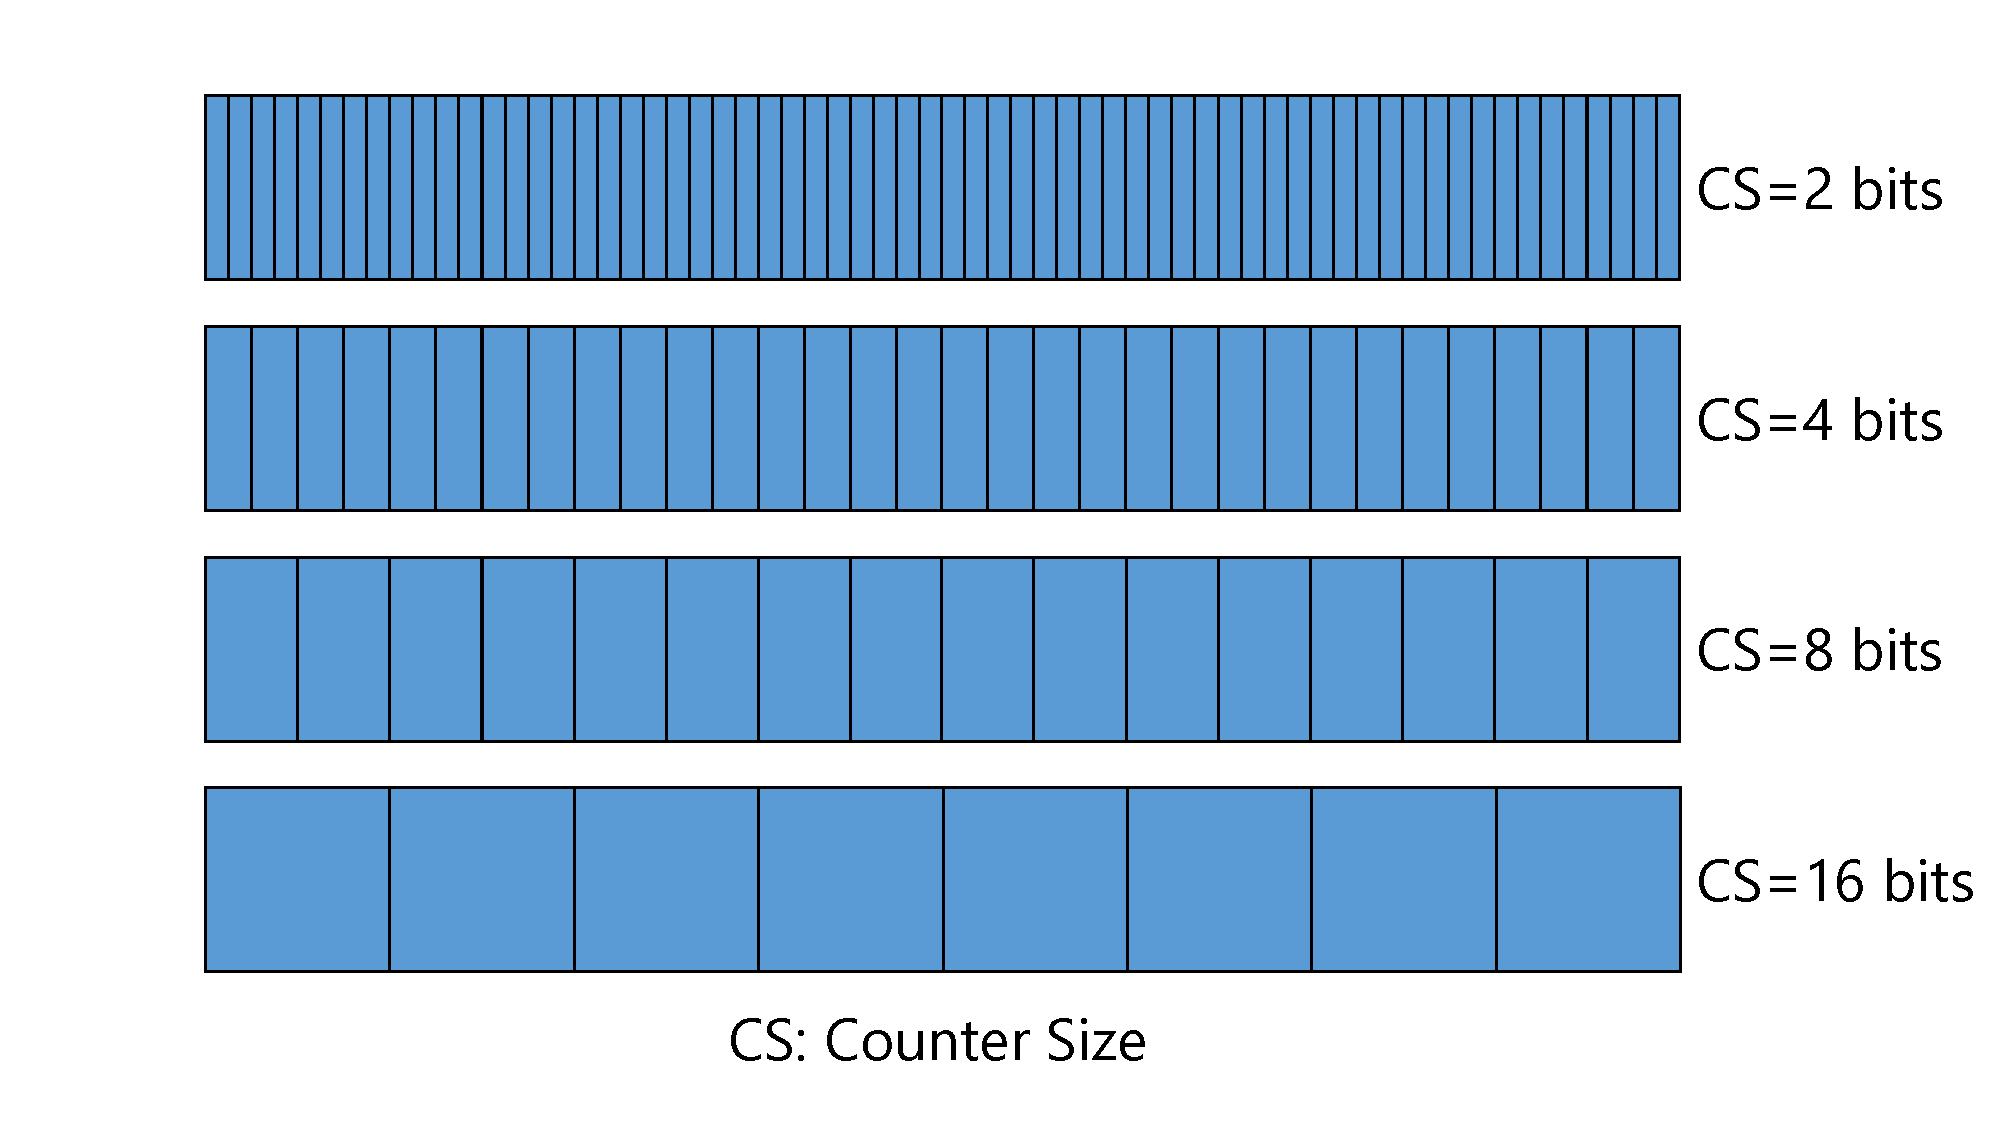
\includegraphics[width=3.5in]{cdv1}
	\caption{The structure of a sketch using the first version of \fname.} 
	\label{draw:version1}
\end{figure}

\presub
\subsubsection{Version 2} \postsub

Based on the first version of our unbalanced parameter setting technique, we can make further improvements on other parameters.
As mentioned above, the distribution of item frequencies will affect the performance of the first version of unbalanced parameter setting technique greatly.
Therefore, we should also take the parameter width into account.

\noindent\textbf{Technical content: }For different distributions of item frequencies, there are different suitable parameter settings. If the percentage of \texttt{cold items} decreases, the width of arrays with small counter size should decrease, and accordingly the width of arrays with larger counter size should increase. If that percentage increases, then the width of arrays with small counter size should increase, and that of arrays with larger counter size should decrease.
Therefore, we should allocate different widths for different arrays based on the distribution.
For example, as shown in Figure \ref{draw:version2}, there are 4 arrays in a sketch, and these 4 arrays have a counter size of 2 bits, 4 bits, 8 bits and 16 bits, respectively.
When the degree of nonuniformity of the dataset is high, then the total number of bits in the first array increases while that in the last array becomes smaller.
When the degree of nonuniformity is small, then the total number of bits in the last array increases.
It resembles cell proliferation and cell apoptosis: when there are enough nutrition, cells will proliferate; and when lack of nutrition, some cells will die.
\textit{The key point of this technique is to use the nonuniformity of past data streams to determine the parameter settings.}

\begin{figure}[htbp]
	\centering
	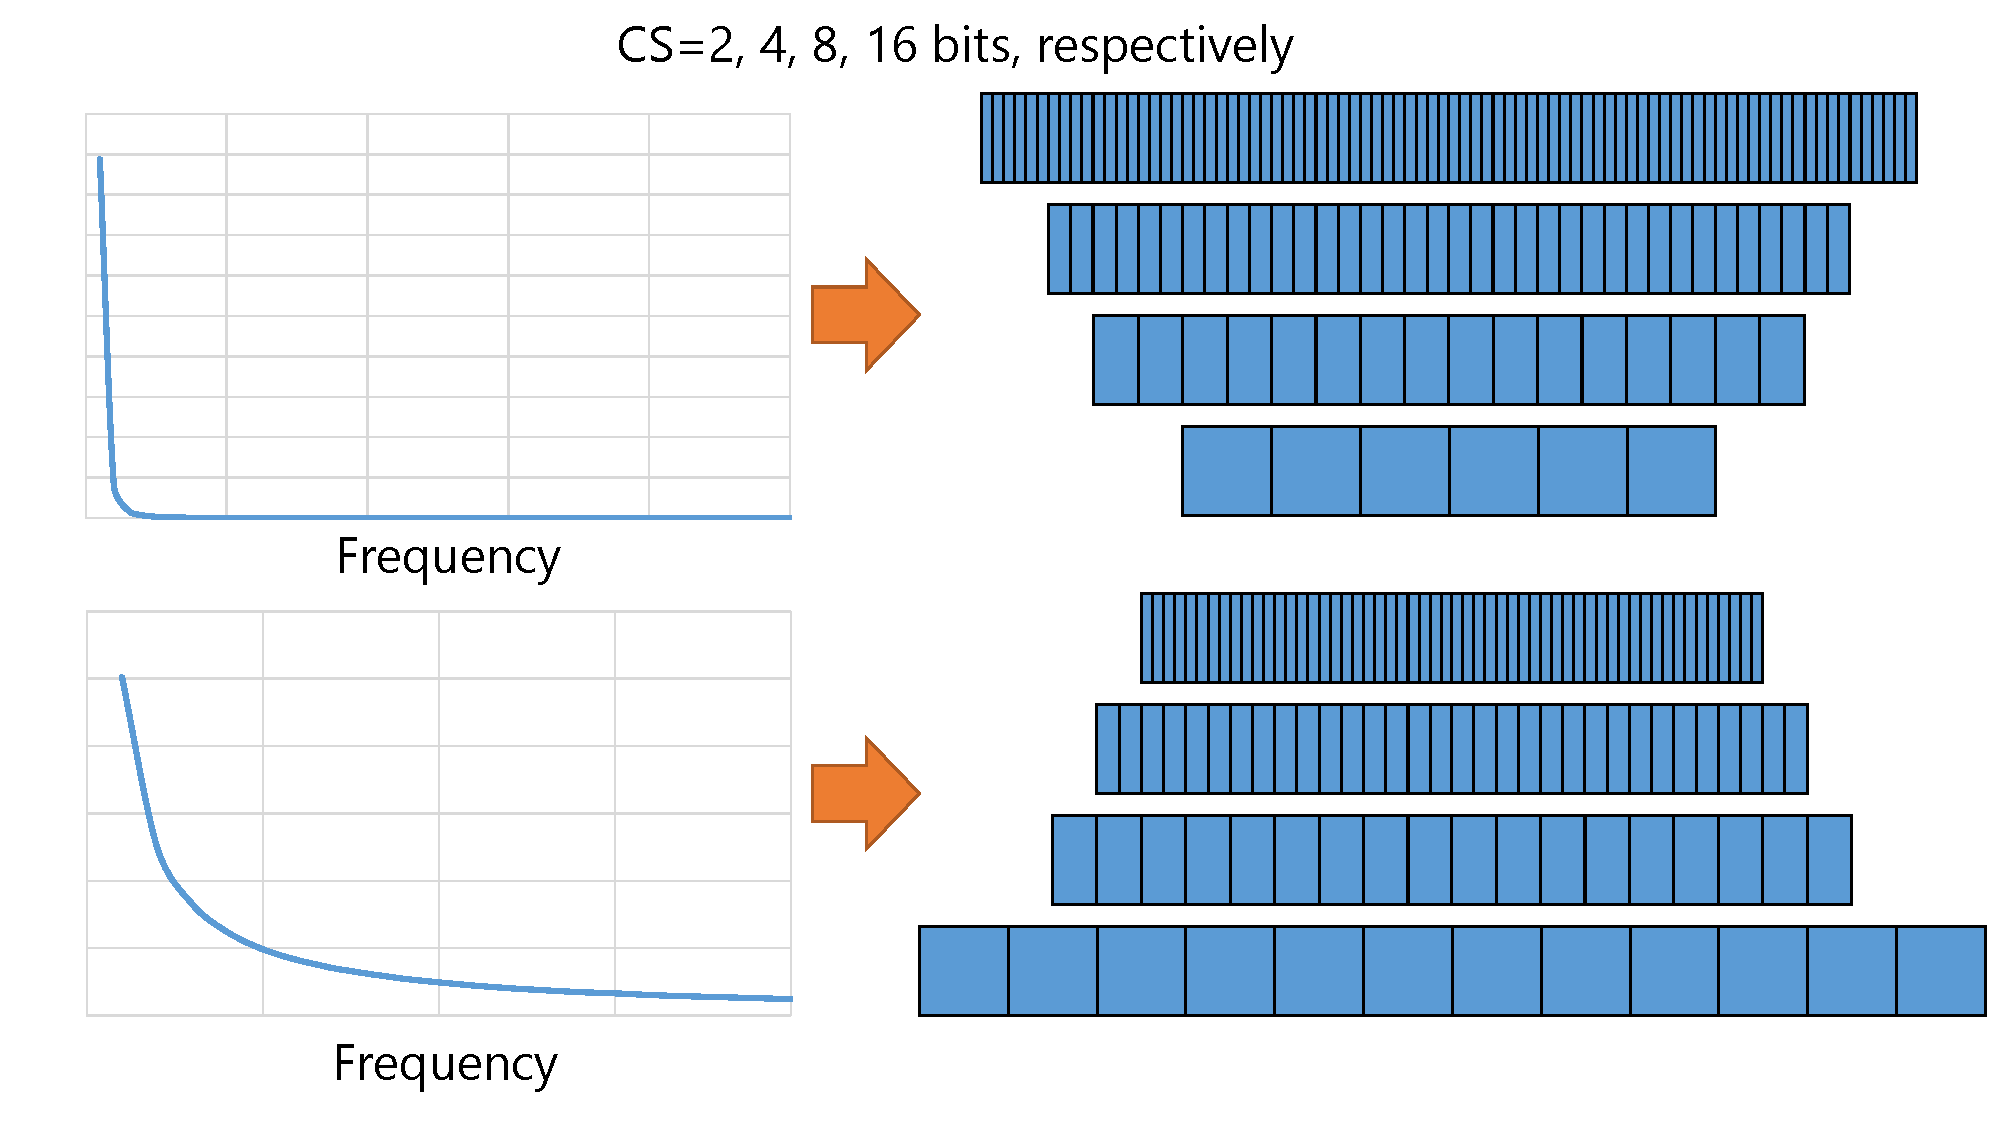
\includegraphics[width=3.5in]{cdv2}
	\caption{The structure of a sketch using the second version of \fname.} 
	\label{draw:version2}
\end{figure}


\noindent\textbf{Analysis: }This version of unbalanced parameter setting can fit the distribution of data streams, so that it can almost achieve the best accuracy as long as there are no drastically changes in the distribution.
However, there is still another problem unsolved.
This version cannot handle counter overflows properly which can lead to low accuracy, especially for \texttt{hot items}.
To address this problem, we propose our second technique in the next part.

\presub
\subsection{Technique II: Overflow Skip} \postsub

In this part, we present our second technique, named \textit{Overflow Skip}.
This technique is aimed to handle counter overflows properly in order to prevent low accuracy for \texttt{hot items}.
If we simply use the same query algorithms as conventional sketches like CM sketches, we will get illogical results.
For example, if we are using a CM sketch with 4 arrays as mentioned above, and there is an item $e$ has a frequency of 10000. The item $e$ is mapped to 4 counters in the sketch, \ie, $A_1[h_1(e)] \dots A_4[h_4(e)]$. When querying the item $e$, we should report the minimum value of these 4 counters. However, the counter $A_1[h_1(e)]$ has a size of only 2 bits, and thus the value in this counter is only 3 due to the counter overflow.
Therefore, we will get an estimated frequency of 3.
Obviously, it is illogical and leads to huge errors.
To address this problem, we use Overflow Skip technique to handle overflows.
\textit{When querying an item, we will get $d$ mapped counters, where $d$ represents the number of arrays in a sketch. If a counter overflows, we will treat the counter as a flag instead of a meaningful frequency, and omit its value when reporting the minimum value among all these $d$ counters.}
For example, as shown in Figure \ref{draw:os}, we are using a CM sketch width 4 arrays as mentioned before.
When querying an item $e$, it is mapped to 4 counters with values of 3, 15, 18 and 41.
As the first counter and the second counter overflow, their values are omitted.
Therefore, we report the estimated frequency of 18 instead of 3.
The pseudocode of this technique applying to the CM sketch is presented in Algorithm \ref{alg:os}.

\begin{figure}[htbp]
	\centering
	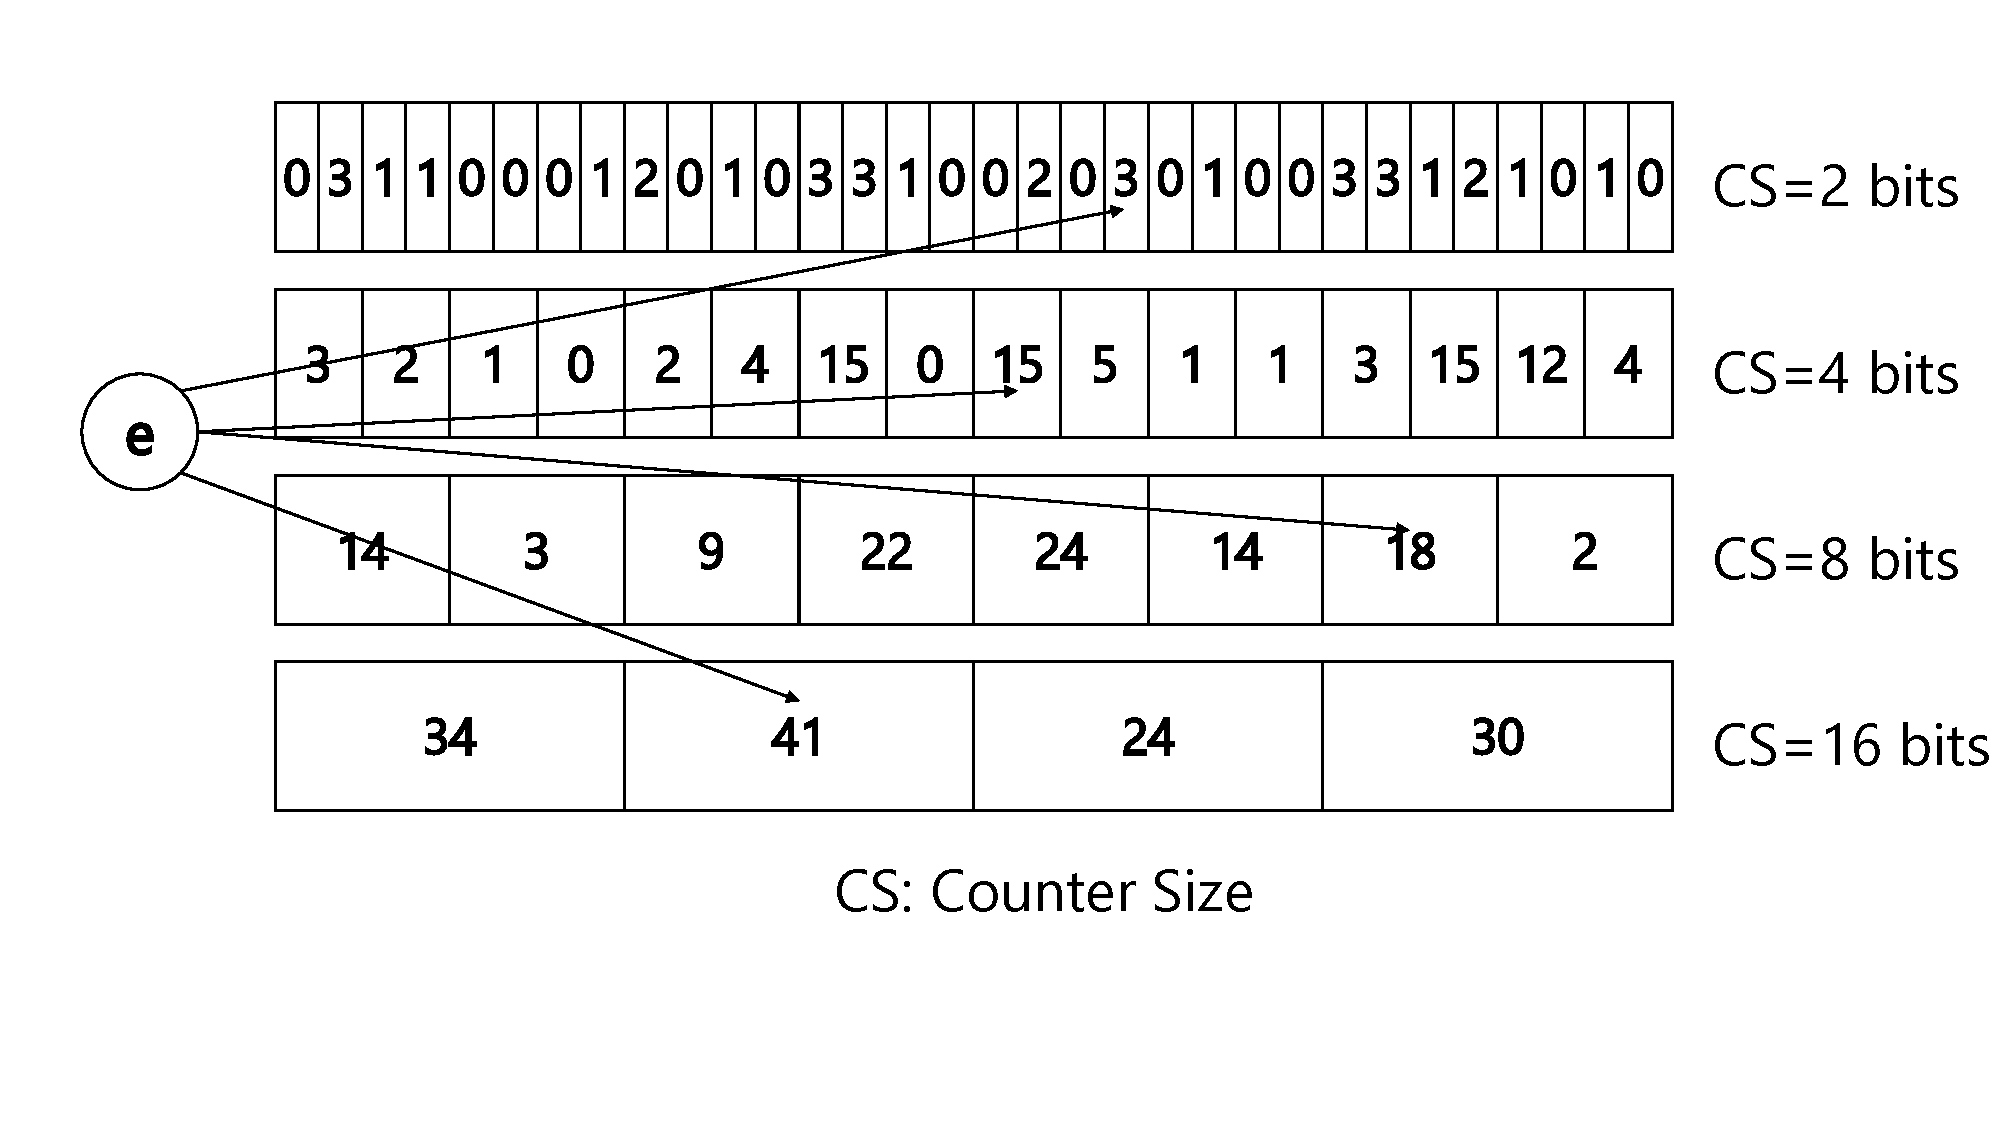
\includegraphics[width=3.5in]{os}
	\caption{The overflow skip technique.} 
	\label{draw:os}
\end{figure}

\begin{algorithm}[h]
	\caption{Query process using the overflow skip technique}
	\label{alg:os}
	% \begin{algorithmic}[1]
	% \Require
	\KwIn{ $e$: an arbitrary item; $A$: a CM sketch; $b$: the counter size of each array}
	% \Ensure
	\KwOut{The estimated frequency of $e$}
%	Procedure {$Query$($e$, $A$)}
	
	$min=MAX\_VALUE$\;
	\For{$j=1$,$j \leqslant d$, $j++$}
	{
		\If{$A_i[h_i(e)]<2^{b_i}-1$}
		{
			\If{$min>A_i[h_i(e)]$}
			{
				$min=A_i[h_i(e)]$\;
			}
		}
	}
	return $min$\;
%	$min=MAX\_VALUE$\;
%	\For{$i=1$;$i\leqslqnt d$;$i++$}
%	{
%		\If{$A_i[h_i(e)]$ overflows}
%		{
%			continue\;
%		}
%	}
\end{algorithm}

\presub
\subsection{Cost Analysis} \postsub

In this part, we give a brief analysis to prove that our \aname~technique is free of extra costs.

\noindent\textbf{Memory access: }For a CM sketch without using our technique, the number of memory accesses for each insertion process or each query process is $d$, the number of arrays in the sketch. After using our \aname~technique, it also requires $d$ memory accesses for each insertion and query process, since each counter can be accessed with one single memory access even if the counter size varies from different arrays. Therefore, there are no extra memory access for CM sketches after using our technique.
This conclusion can also be applied to other sketches, whose analysis is omitted due to space limitation.

\noindent\textbf{Computational complexity: }Except for the amount of computations needed for sketches without using our technique, sketches using our technique requires at most 2 displacement operations for each mapped counter when performing insertion or query processes.
This extra amount of computations is far smaller than that required before using our technique, including hash function computations.
Therefore, our \aname~technique almost introduce no extra computational complexity.

\noindent\textbf{Others: }Our \aname~technique also does not introduce other extra costs. For example, the CM sketch and the CU sketch suffer from no under-estimation errors, and so do these sketches after using our technique. The proof of this will be presented in the next section.
Furthermore, the CM sketch after using our technique also supports deletion operations like those without using our technique.
	\presec
\section{Analysis} \postsec

In this section, we carry out comprehensive mathematical analysis for our \aname~technique.
We mainly focus on the correct rate and the error bound of the CM sketch after using our \aname~technique.
We also give a proof of no under-estimation error for the CM sketch after using our technique.
We call the CM sketch after using this technique the \ccm.

\presub
\subsection{Proof of No Under-estimation Error} \postsub

In this subsection, we prove that \ccm has no under-estimation error. Under-estimation error means that \emph{the querying value is smaller than the real frequency.} 
As the insertion may make counters overflow and become invalid, the set of valid arrays for the inserted item change over time. 
For item $e$, let $S_n$ denote the set of indexes of valid arrays after $n^{th}$ insertion, and let $a_i$ denote the index of corresponding counter of item $e$ in $i^{th}$ array.
By mathematical induction, we prove that if there is at least one valid array after $n^{th}$ insertion of item $e$, i.e. $S_n \neq \emptyset$, the \ccm~has no under-estimation error.

\noindent\textbf{Base case: } Suppose $n = 1$. 
After first insertion of item $e$, all valid counters of $e$ increase by one, so $min_{i\in S_1}\{A_i[a_i]\} \ge 1$. 
The query result won't be smaller than $1$, which means the \ccm~has no under-estimation error in this case. 

\noindent\textbf{Inductive hypothesis: } Assume when $n = k (k \ge 1)$, the \ccm~has no under-estimation error, i.e. $min_{i\in S_k}\{A_i[a_i]\} \ge k$.

\noindent\textbf{Inductive step: } Suppose $n = k + 1$. 
As $S_{k+1}\subseteq S_k$, we know before the insertion, $min_{i\in S_{k+1}}\{A_i[a_i]\} \ge k$. After the insertion of item $e$, all valid counters of $e$ increase by one, so $min_{i\in S_{k+1}}\{A_i[a_i]\} \ge k+1$. 
The query result won't be smaller than $k+1$, which means the \ccm~has no under-estimation error in this case. 

In conclusion, the \ccm~has no under-estimation error.

\presub
\subsection{Correct Rate of the \ccm} \postsub

Given a multiset with N distinct items, let $e_i$ denote the $i^{th}$ item, and $f_i$ denote its frequency. If the frequency exceeds the capacity of some counters, these counters will overflow and become invalid. Without loss of generality, we assume $b_1 \le b_2 \le \dots \le b_d$, and define
\begin{equation*}
E_i=
\begin{cases}
\{e_j|1\le f_j < 2^{b_1}-1, 1\le j \le N \} & {i=1}\\
\{e_j|2^{b_{i-1}}-1\le f_j < 2^{b_i}-1, 1\le j \le N\} & {1 < i \le d}
\end{cases}
\end{equation*}

For items in $E_i$, their corresponding counters located in $1 \sim i-1$ arrays will overflow and become invalid.

\begin{thm}
Let $p_i$ denote the probability that one arbitrary counter in $i^{th}$ array stores the accurate value of its corresponding item. 
$p_i$ equals to the probability that no collision happens in in one certain counter in $i^{th}$ array :
\begin{equation}
p_i=(\frac{w_i-1}{w_i})^{N-1} 
\end{equation}

\end{thm}
According to the uniform property of hash function $h_i(.)$, this equation is obvious.

\begin{thm}
Let $P_i$ denote the probability that items in $E_i$ can get an accurate result when querying the \ccm. Then
\begin{equation}
P_i=1-\prod_{j=i}^{d}(1-p_j)
\end{equation}
\end{thm}

\begin{proof}
For item $e \in E_i$, if $1\le j<i$, $e$'s corresponding counters in $j^{th}$ array will overflow and the probability that it can't provide the accurate result is $1$; 
if $i\le j \le d$, The probability that $e$ couldn't get the accurate result from its corresponding counter in $j^{th}$ array is $1-p_j$. 
The \ccm~ fails to report an accurate result when the corresponding counters in all arrays fail to provide the accurate result, whose probability is 
$$  P_{fail}=\prod_{j=1}^{i-1}1 \prod_{j=i}^{d}(1-p_j)=\prod_{j=i}^{d}(1-p_j) $$
Therefore, the probability that \ccm~can report the accurate result of $e$ is $1-P_{failed}$.
\end{proof}

\begin{thm}
Let $C$ denote the correct rate of the \ccm. Then
\begin{equation}
C=\sum_{i=1}^{d}\frac{|E_i|P_i}{N}
\end{equation}
\end{thm}

\presub
\subsection{Error Bound of the \ccm} \postsub

Without loss of generality, assume $b_1 \le b_2 \le \cdots \le b_d$. 
\begin{thm}
For an arbituary item $e_i$, assume its corresponding counter in $t^{th}$ array doesn't overflow while ones in array $1 \sim t-1$ overflow. 
Without loss of generality, assume all its corresponding counters in array $t \sim d$ don't overflow. 
Let $\hat{f_i}$ denote its estimated frequency and $f_i$ denote its real frequency. 
Let $N$ denote the number of distinct items and $V$ denote the sum of all items' real frequency, i.e. $V=\sum_{k=1}^{N}f_i$.
Given a small variable $\epsilon$, we have the following guarantee with probability at least $1-(\epsilon w_d) ^{d-t+1}$:
\begin{equation}
\hat{f_i} \le f_i + \epsilon V
\end{equation}
\end{thm}

\begin{proof}
We define an indicator variable $I_{i,j,k}$ that is 1 if $h_j(e_i)=h_j(e_k)$, and $0$ otherwise. 
Due to the independence of hash functions, the expectation of this indicator variable is:
\begin{equation}
E(I_{i,j,k})=Pr[h_j(i)=h_j(k)]=\frac{1}{w_j}\le \frac{1}{w_d}
\end{equation}
We define the variable $X_{i,j}$ as $X_{i,j}=\sum_{k=1}^{N}I_{i,j,k}f_k$.
$X_{i,j}$ reflects the expectation of the error caused by the collisions happening in a counter of $j^{th}$ array. Let $R(A_i[j])$ denote the report value of $A_i[j]$, then we have
\begin{equation}
R(A_i[h_j(e_k)])=f_k+X_{i,j}
\end{equation}
The expectation of $X_{i,j}$ is:
\begin{equation}
E(X_{i,j})=E(\sum_{k=1}^{N}I_{i,j,k}f_k)=\sum_{k=1}^{d}f_k E(I_{i,j,k}) \le \frac{V}{w_d}
\end{equation}
Then, by the Markov inequality, we have:
\begin{equation}
\begin{aligned}
&Pr\left[\hat{f_i} \ge f_i+\epsilon V\right] \\
&= Pr\left[\forall _{j \ge t .~} R(A_j[h_j(e_i)])\ge f_i+\epsilon V\right] \\
&= Pr\left[\forall _{j \ge t .~} f_i + X_{i,j}\ge f_i+\epsilon V\right] \\
&= Pr\left[\forall _{j \ge t .~} X_{i,j}\ge \epsilon V\right] \\
&= Pr\left[\forall _{j \ge t .~} \frac{X_{i,j}}{E(X_{i,j})}\ge \epsilon w_d\right] \\
&\le \left\{E\left[\frac{X_{i,j}}{E(X_{i,j})}\right]/(\epsilon w_d)\right\}^{d-t+1} \\
&= (\epsilon w_d)^{d-t+1}
\end{aligned}
\end{equation}
\end{proof}



	\presec
\section{Experimental Results} \postsec

	\presec
\section{Conclusion} \postsec

Sketches are widely used in many applications due to their high accuracy, memory efficiency and fast speed.
However, many real datasets are non-uniform, and sketches are not accurate enough for these datasets because of high probability of hash collisions.
To address this issue, in this paper, we propose a novel technique for sketches, named \fname~(\aname), which enables exisiting sketches to achieve higher accuray with few extra costs.
The key idea of our \aname~technique is to use different parameters like width and counter size in different arrays in a sketch.
We apply our technique to several typical sketches, including CM sketches and CU sketches.
We also conduct comprehensive mathematical analysis and extensive experiments to prove that sketches perform better after using our technique.
Experimental results show that our \aname~technique is ...
We believe our \aname~technique can be widely applied to many sketches.
	
	\balance
	\bibliographystyle{unsrt}
	\bibliography{InputFiles/reference}
\end{document}


